
\subsection{Węzły}
Matematyczne węzły można traktować jako model elastycznej oraz pozbawionej grubości liny, której luźne końce zostały ze sobą połączone.
Sugeruje to przyjęcie naiwnej definicji:

\begin{definition}[węzeł (prawie)]
\index{węzeł}%
    Ciągłe oraz różnowartościowe odwzorowanie $S^1 \to \R^3$ nazywamy węzłem.
\end{definition}

Takie rozwiązanie nie jest doskonałe, ponieważ oprócz pożądanych (cokolwiek to znaczy) węzłów, obejmuje wiele innych, patologicznych obiektów takich jak ten z~rysunku \ref{fig_wild_knot}.

\begin{figure}[H]
    \centering
\begin{comment}
    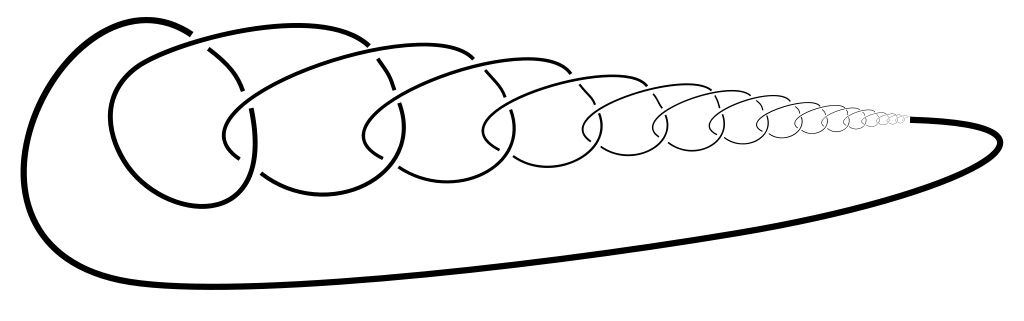
\includegraphics[height=0.14\linewidth]{wild_knot.png}
\end{comment}
    \caption[caption-wild-knot]{Węzeł dziki, źródło: Wikimedia{\footnotemark}}
\index{węzeł!dziki}%
\label{fig_wild_knot}%
\end{figure}
\footnotetext{\url{https://upload.wikimedia.org/wikipedia/commons/2/2f/Wildknot.svg}}

Zamiast wyjaśnić, jakie są jego niepożądane właściwości, podamy od razu dobrą definicję.

\begin{definition}[węzeł]
    Różnowartościowe włożenie $S^1 \to \R^3$, którego pochodna istnieje wszędzie i~nie znika nigdzie, nazywamy węzłem.
\end{definition}

\begin{example}[niewęzeł]
    Węzeł zadany w przestrzeni $\R^3$ parametrycznie $(\sin \theta, \cos \theta, 0)$ dla $\theta \in [0, 2\pi]$ nazywamy niewęzłem i oznaczamy $\SmallUnknot$.
\end{example}

Potrzeba jeszcze matematycznego opisu manipulacji, jakim możemy poddawać sznur trzymany w~ręce.
Izotopia jest niewłaściwym narzędziem do tego celu: powiedzielibyśmy, że dwa węzły $K_1, K_2$ sa izotopijne, jeśli istnieje ciągła funkcja
\begin{equation}
    F \colon S^1 \times [0, 1] \to \R^3
\end{equation}
taka, że $K_1 = F(-, 0)$ jest pierwszym, zaś $K_2 = F(-,1)$ drugim węzłem (funkcję $F$ nazywa się izotopią).
Tym razem źródło problemów można wskazać jawnie.
Dowolny zaplątany fragment z węzła można usunąć wykonując sztuczkę Alexandera (ponieważ jak powiedziałyby mądre głowy, ,,przestrzeń homeomorfizmów dysku w siebie $D^{n+1} \to D^{n+1}$, które zgadzają się z odwzorowaniem tożsamościowym na brzegu dysku -- sferze $S^n$, jest spójna''):
\index[persons]{Alexander, James}%
\index{sztuczka!Alexandera}%

\begin{comment}
\begin{figure}[H]
    \centering
    \fbox{\begin{minipage}[b]{.12\linewidth}
        \centering
        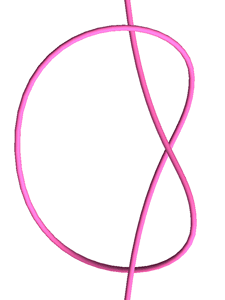
\includegraphics[width=\linewidth]{../data/alexander-trick/0.png}
        \subcaption{$t = 0$}
    \end{minipage}}\,\,
    \fbox{\begin{minipage}[b]{.12\linewidth}
        \centering
        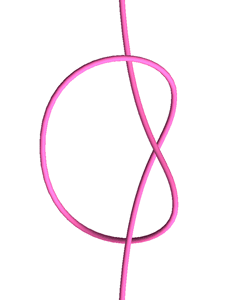
\includegraphics[width=\linewidth]{../data/alexander-trick/1.png}
        \subcaption{$t = 1/4$}
    \end{minipage}}\,\,
    \fbox{\begin{minipage}[b]{.12\linewidth}
        \centering
        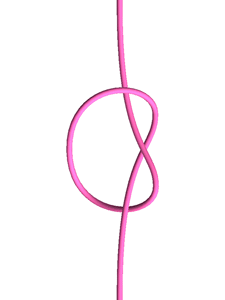
\includegraphics[width=\linewidth]{../data/alexander-trick/2.png}
        \subcaption{$t=1/2$}
    \end{minipage}}\,\,
    \fbox{\begin{minipage}[b]{.12\linewidth}
        \centering
        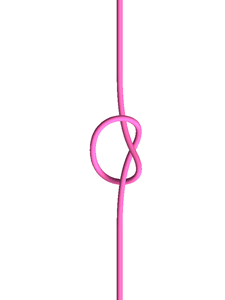
\includegraphics[width=\linewidth]{../data/alexander-trick/3.png}
        \subcaption{$t=3/4$}
    \end{minipage}}\,\,
    \fbox{\begin{minipage}[b]{.12\linewidth}
        \centering
        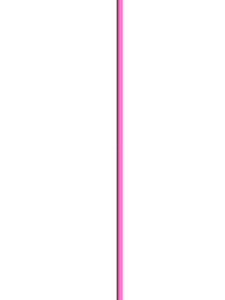
\includegraphics[width=\linewidth]{../data/alexander-trick/4.png}
        \subcaption{$t = 1$}
    \end{minipage}}
    \caption[caption-alexander-trick]{Sztuczka Alexandera}
\end{figure}
\end{comment}

W podobny sposób moglibyśmy przekształcić dowolny węzeł w~niewęzeł.
Teoria, w~której wszystkie obiekty są takie same, nie jest zbyt ciekawa.
Od izotopii należy wymagać gładkości albo lokalnej płaskości,
% https://math.stackexchange.com/questions/1311865/equivalence-of-knots-ambient-isotopy-vs-homeomorphism
co zdaje się prowadzić do pojęcia izotopii otaczającej, która uwzględnia nie tylko sam węzły, ale też to, jak leżą w otaczającej je przestrzeni.

% DICTIONARY;isotopy;izotopia;-
% GLOSSAIRE;isotopie;izotopia;-
% DICTIONARY;ambient;otaczająca;izotopia
% GLOSSAIRE;ambiante;otaczająca;izotopia
\begin{definition}[izotopia otaczająca]
    \index{izotopia otaczająca}%
    Niech $K_1, K_2 \colon N \hookrightarrow M$ będą włożeniami dwóch rozmaitości $N, M$.
    Ciągłe odwzorowanie $F \colon M \times [0,1] \to M$ spełniające następujące warunki:
    \begin{enumerate}
        \item funkcja $F(-, 0)$ jest odwzorowaniem tożsamościowym,
        \item każda z~funkcji $F(-, t)$ jest homeomorfizmem,
        \item złożenie $F(-, 1)$ z~pierwszym włożeniem $K_1$ daje drugie włożenie $K_2$
    \end{enumerate}
    nazywamy izotopią otaczającą przenoszącą włożenie $K_1$ na $K_2$.
\end{definition}

W~topologii rozważa się włożenia dowolnych rozmaitości, nam wystarczy jeden szczególny przypadek $N = S^1$ oraz $M = \R^3$.
Intuicyjnie, funkcja $F$ zniekształca przestrzeń $\R^3$ tak, że w~chwili początkowej $t = 0$ widzimy pierwszy, zaś w~chwili końcowej $t = 1$ drugi węzeł.
Izotopia otaczająca nie pozwala na ściąganie zaplątanych fragmentów do punktu.

\begin{definition}
    Dwa węzły są równoważne wtedy i tylko wtedy, gdy istnieje pomiędzy nimi izotopia otaczająca.
\end{definition}

Znając już izotopię otaczającą, można podać alternatywny opis węzłów:

% DICTIONARY;knot;węzeł;-
% GLOSSAIRE;nœud;węzeł;-
% DICTIONARY;tame;poskromiony;węzeł
% GLOSSAIRE;lisse/régulier;poskromiony;węzeł
% DICTIONARY;wild;dziki;węzeł
% GLOSSAIRE;sauvage;dziki;węzeł
\begin{definition}[węzeł]
\index{węzeł!poskromiony}%
\label{def:knot}%
    Gładkie włożenie $S^1 \hookrightarrow \R^3$ otaczająco izotopijne z~zamkniętą łamaną bez samoprzecięć nazywamy węzłem poskromionym.
\end{definition}

Czasami wygodniej jest rozpatrywać węzeł jako włożenie $S^1 \hookrightarrow S^3$ albo dopuścić do myśli węzły nieposkromione.
Ale jeśli nie zaznaczono inaczej, nie robimy tego: pisząc węzeł mamy na myśli poskromione włożenie w przestrzeń $\R^3$, nie $S^3$.

Formalnie węzły to pewne odwzorowania, więc prawidłowym sposobem na zapisanie, że są izotopijne (czyli dla nas: równe), jest $K_1 \cong K_2$.
Ponieważ nie prowadzi to do problemów, będziemy jednak stosować zapis $K_1 = K_2$.
Jednocześnie często węzeł jako odwzorowanie nie będzie odróżniany od obrazu tego odwzorowania.

Istnieje jeszcze jedna, konkurencyjna definicja węzłów równoważnych:

\begin{proposition}
\label{def:equivalent_knots_2}%
    Dwa węzły są równoważne wtedy i~tylko wtedy, gdy jeden z~nich jest obrazem drugiego przez zachowujący orientację homeomorfizm $\R^3 \to \R^3$.
\end{proposition}

\begin{proof}
    Podany niżej dowód pochodzi z~książki ,,Topology from the differentiable viewpoint'' Johna Milnora.
\index[persons]{Milnor, John}%
    Musimy pokazać, że dyfeomorfizm $f \colon \R^m \to \R^m$ jest gładko izotopijny z~identycznością.
    Translacje są izotopiami, więc bez straty ogólności zakładamy, że $f(0) = 0$.
    Pochodna $f$ w~zerze jest dana wzorem $\mathrm{d}f_0(x) = \lim_{t \to 0} f(tx) /t$, więc
    \begin{equation}
        F(x, t) = \begin{cases}
            \mathrm{d}f_0(x) & t = 0 \\
            f(tx) / t & 0 < t \le 1
        \end{cases} .
    \end{equation}
    stanowi naturalną definicję izotopii $F \colon \R^m \times [0, 1] \to \R^m$.
    Funkcja $f$ zapisuje się na mocy lematu Hadamarda jako suma $x_1 g_1(x) + \ldots + x_mg_m(x)$, gdzie funkcje $g_i$ są gładkie, więc funkcja $F$ też jest gładka, co jakoś kończy dowód.
\index{lemat Hadamarda}%    
\end{proof}

Milnor zauważa, że istnieje dyfeomorfizm $S^6 \to S^6$ stopnia $+1$, który nie jest gładko izotopijny z~identycznością!
\index[persons]{Milnor, John}%

\begin{remark}[John Willard Milnor]
    Matematyk amerykański urodzon w 1931 roku w Orange, New Jersey.
    Odkrył egzotyczną 7-wymiarową sferę (czyli zwykłą sferę z niezwykłą strukturą różniczkową) w 1956 roku, za co został później odznaczon medalem Fieldsa.
    Obalił Hauptvermutung pięć lat później: hipotezę Steinitza i Tietzego z 1908 roku, że każde dwie triangulacje przestrzenii mają kombinatorycznie równoważne podpodziały.
    Do jego zainteresowań należą topologia różniczkowa, algebraiczna K-teorią, ale też algebry Hopfa, grupy Liego i holomorficzne układy dynamiczne.
    W~świecie węzłów jest znany przez wprowadzenie niezmienników $\mu$ Milnora, które uogólniają grupę podstawową dopełnienia oraz pewne wyniki dotyczące hipotezy plastrowo-taśmowej.
\end{remark}
\index{niezmiennik $\mu$ Milnora}%
\index{hipoteza plastrowo-taśmowa}%
\index[persons]{Milnor, John}%

